\section{Processi primari}

\subsection{Fornitura}
	
	\subsubsection{Scopo}
		Lo scopo di questo $processo_G$ è di trattare i termini e le norme, dalle più triviali alle più importanti, che tutti i componenti del gruppo SWEefty sono tenuti a rispettare per diventare fornitori dell'azienda IKS s.r.l e dei committenti Prof. Tullio Vardanega e Prof. Riccardo Cardin.
	\subsubsection{Attività} 
		\paragraph{Studio di fattibilità} \mbox{} \\
		Sono state organizzate diverse riunioni al fine di permettere ai membri del team di scambiarsi opinioni sui capitolati proposti. 
		Abbiamo valutato il capitolato secondo diversi criteri:
		\begin{itemize}
			\item \textbf{Dominio tecnologico:} E' stata presa in considerazione la conoscenza attuale delle tecnologie richieste per portare a termine i vari capitolati, in base
			anche a esperienze passate avute con problemi simili.
			\item \textbf{Individuazione rischi:} sono state analizzate le varie difficoltà che si potrebbero incontrare durante la realizzazione dei vari capitolati considerando 
			in modo particolare la mancanza di conoscenze adeguate relative alle tecnologie necessarie per realizzare i capitolati.
		\end{itemize}  
		\paragraph{Piano di Progetto} \mbox{} \\
		Il \emph{Project Manager} affiancato dall' \emph{Amministratore} dovrà stilare un piano da seguire per la realizzazione del progetto.
		Il documento dovrà rispettare e seguire i seguenti punti:
		\begin{itemize}
		\item \textbf{Analisi dei rischi:} si analizzano nel dettaglio i rischi che si potrebbero presentare durante lo svolgimento del progetto, capendo con quale probabilità potrebbero accadere e qual è il livello di gravità di ogni rischio.
		\item \textbf{Pianificazione:} si pianificano le attività da svolgere nel corso del progetto fornendo delle scadenze temporali precise.
		\item \textbf{Preventivo:} si stima, secondo la pianificazione, la quantità di lavoro necessaria per portare a termine ogni fase, in modo tale da riuscire a proporre un preventivo finale per il costo totale del progetto.
		\end{itemize} 
		
		\paragraph{Piano di Qualifica} \mbox{} \\
		Al \emph{Verificatore} è assegnato il compito di scegliere un metodo per la $verifica_G$ e $validazione_G$ del materiale realizzato dal team.
		Il documento deve contenere:
		\begin{itemize}
		\item \textbf{Metodo di verifica:} vengono stabilite le procedure di controllo sulla qualità di processo e di prodotto. 
		\item \textbf{Metriche:} è necessario stabilire delle metriche oggettive per i documenti e i processi software.
		\item \textbf{Gestione della revisione:} si devono stabilire delle modalità per comunicare le anomalie e le procedure per controllare la qualità di processo;
		\item \textbf{Pianificazione collaudo:} è necessario definire dettagliatamente le metodologie di collaudo del progetto.
		\item \textbf{Resoconto attività verifica:} alla fine di ogni attività svolta si devono riportare le metriche relative e un resoconto sulla verifica effettuata.
		\end{itemize}
	
\subsection{Sviluppo}
	\subsubsection{Scopo}
	Questa sezione affrontà le attività e i compiti svolti dal gruppo al fine di produrre il software richiesto dall'azienda IKS Srl.
	
	\subsubsection{Aspettative}
	Al fine di implementare correttamente questa attività vi sono le seguenti aspettative:
	\begin{itemize}
		\item Realizzare un prodotto software conforme alle richieste del proponente
		\item Realizzare un prodotto software che soddisfi i test di verifica
		\item Realizzare un prodotto software che soddisfi i test di validazione
		\item Fissare degli obiettivi di $sviluppo_G$
		\item Fissare eventuali vincoli tecnologici
		\item Fissare i vincoli di design
	\end{itemize}
	
	\subsubsection{Descrizione}
	Il processo di sviluppo si svolge in accordo con lo standard ISO/IEC 12207.Pertanto si compone delle seguenti attività:
	\begin{itemize}
		\item Analisi dei requisiti
		\item Progettazione
		\item Codifica
	\end{itemize}
	
	\subsubsection{Attività}
		\paragraph{Analisi dei requisiti}
			\subparagraph{Scopo}
			Lo scopo di questa analisi è quella di elencare nel modo più preciso possibile, tutti i requisiti del progetto. 
			I requisiti sono estrapolati da diverse fonti:
				\begin{itemize}
				\item Specifica del capitolato 
				\item Incontri tenuti direttamente con il proponente
				\item Casi d'uso
			\end{itemize}
		    Dopo aver svolto questo processo viene stilato in modo formale un documento di analisi chiamato \textit{Analisi dei Requisiti v1.0.0}.
		    Quest'ultimo è steso dagli \emph{Analisti} e contiene una lista dei requisiti e dei casi d'uso.
		    In questo modo sarà possibile effettuare e definire dei test di superamento del software. 
			\subparagraph{Aspettative}
			L'obiettivo di questa attività è quello di definire in modo formale e dettagliato tutti i requisiti richiesti dal proponente.
			\subparagraph{Descrizione}
			Nel documento inerente a quest'analisi sono specificati i requisiti analizzati.
			Il metodo utilizzato per l'analisi dei requisiti è quella dei casi d'uso.
			\subparagraph{Casi d'uso}
			\subparagraph{Codice identificativo}
			\subparagraph{Requisiti}
			\subparagraph{Codice identificativo}
			\subparagraph{UML}
			I diagrammi UML devono essere realizzati usando la versione del linguaggio \textit{v2.0}
			
			
		\paragraph{Progettazione}
			\subparagraph{Scopo}
			\mbox{}\\
			L'attività di Progettazione  ha lo scopo di definire e descrivere la progettazione ad alto livello dell'architettura del prodotto richiesto e specificarla descrivendo la progettazione di dettaglio. \\
			Il responsabile di questa attività è il \emph{$Progettista_G$} che deve redarre la \texttt{Specifica Tecnica} e la \texttt{Definizione di Prodotto} in funzione dei requisiti delineati nell'\texttt{Analisi dei Requisiti} in modo da permettere di definire le linee guida da seguire durante l'attività di codifica.
			Per fare ciò deve avere una profonda conoscenza dell'intero processo di sviluppo del software.
			Solo in questo modo possono:
			\begin{itemize}
				\item progettare un software con le caratteristiche di qualità specificate nella fase di analisi e specifica dei requisiti;
				\item effettuare modifiche senza che la struttura del software già costruita debba essere messa nuovamente in discussione;
				\item soddisfare i requisiti di qualità fissati dal committente.
			\end{itemize}
			\subparagraph{Specifica Tecnica}
			\mbox{}\\
			Questo documento deve descrivere la progettazione ad alto livello dell'architettura del software richiesto dal proponente. Inoltre deve provvedere alla progettazione di sistemi di integrazione. 
			Per fare ciò si useranno i seguenti strumenti:
				\begin{itemize}
					\item Diagrammi $UML_G$:\\
					Essi forniscono una rappresentazione molto chiara e compatta dell'intera struttura dell'applicazione che si andrà ad analizzare. In particolare devono essere realizzati i seguenti diagrammi:
					\begin{itemize}
						\item[-] Diagrammi delle classi: illustrano una collezione di elementi dichiarativi di un modello come classi e tipi, assieme ai loro contenuti e alle loro relazioni;
						\item[-] Diagrammi dei $package_G$:  raggruppamento di classi in una unità di livello più alto;
						\item[-] Diagrammi di attività: illustrano il flusso di operazioni relativo ad un'attività. Utilizzati soprattutto per descrivere la logica di un algoritmo;
						\item[-] Diagrammi di sequenza: descrivono una determinata sequenza di azioni dove tutte le scelte sono già effettuate. In pratica nel diagramma non compaiono scelte ne flussi alternativi.
					\end{itemize}
				I diagrammi UML sono realizzati tramite il programma StarUML descritto nella sezione \ref{sec:StarUML}.
					\item $Design Pattern_G$:\\
					Devono essere descritti tramite descrizione e diagramma i design pattern utilizzati.
					\item Tracciamento delle componenti:\\
					Ogni requisito deve riferirsi al componente che lo soddisfa. Per fare ciò si utilizzerà SWEgo, un'applicazione web (descritta nella sezione \ref{sec:SWEgo}) utile nel tracciamento Use Case - Requisiti e nella generazione automatica dei diagrammi dei Casi d'Uso.
					\item Test di integrazione:\\ 
					I Progettisti devono definire delle classi di verifica per verificare che i componenti del sistema funzionino nella maniera prevista.	
				\end{itemize}
			\subparagraph{Definizione di Prodotto}
			\mbox{}\\
			Questo documento deve descrivere la progettazione in dettaglio del sistema, utilizzando i seguenti strumenti:
				\begin{itemize}
					\item Diagrammi $UML_G$\\
					Devono essere realizzati i seguenti diagrammi:
					\begin{itemize}
						\item[-] Diagrammi delle classi;
						\item[-] Diagrammi dei $package_G$;
						\item[-] Diagrammi di attività;
						\item[-] Diagrammi di sequenza.
					\end{itemize}
				I diagrammi UML sono realizzati tramite il programma StarUML descritto nella sezione \ref{sec:StarUML}.
					\item Definizione delle classi\\ 
					Ogni $classe_G$ progettata deve essere descritta con una spiegazione sullo scopo della classe e deve specificare quale funzionalità essa modella. 
					\item Tracciamento classi:\\
					Ogni requisito deve essere tracciato alle classi che lo soddisfano. Per fare ciò si utilizzerà SWEgo, un'applicazione web descritta nella sezione \ref{sec:SWEgo}.
					\item Test di unità:\\
					I Progettisti devono definire i test di unità necessari per verificare che i componenti del sistema funzionino nel modo previsto.
				\end{itemize}
			
			
		\paragraph{Codifica}
			\subparagraph{Scopo} \mbox{} \\
			Questa attività ha come scopo l'effettiva implementazione del prodotto software richiesto. In questa fase dunque si concretizzano attraverso la codifica le funzionalità previste dai requisiti concordati.
			L'attività deve rispettare quando imposto dai documenti \textit{Definizione di prodotto} e \textit{Piano di Qualifica}.
			\subparagraph{Stile di codifica} \mbox{} \\
			Al fine di garantire uniformità all'intera $codebase_G$, ciascun membro del gruppo è obbligato a rispettare le seguenti norme:
			\begin{itemize}
			\item \textbf{Formattazione}: è richiesto l'uso di uno spazio (" ") ove possibile per rendere il codice di facile comprensione.
			Di seguito alcuni  esempi di buona e cattiva formattazione.
\begin{lstlisting}
int a=3; // BAD
int a = 3; // GOOD
int a = 3,b = 5; // BAD
int a = 3, b = 4; // GOOD

getFoo(a,b,c,d); // BAD
getFoo(a, b, c, d); // GOOD

if(a==5){ // BAD
if (a == 5) { // GOOD
\end{lstlisting}
			
			\item \textbf{Indentazione:} sono richiesti 4 spazi (si consiglia di impostare adeguatamente il proprio $IDE_G$), inoltre non sono permessi spazi bianchi o tabulazioni a fine riga.
			
			\item \textbf{Lunghezza linee di codice:} una riga di codice non deve superare i 100 caratteri, in caso contrario spezzare la riga di codice andando a capo.
			
			\item \textbf{Nomi:} i nomi delle funzioni e delle variabili devono essere significativi e devono cominciare con la lettera minuscola e seguire la notazione $camelCase_G$. I nomi delle classi devono avere la prima lettera maiuscola mentre i nomi delle costanti devono essere scritti interamente in maiuscolo.
\begin{lstlisting}
var foo; // BAD
var profiledata // BAD
var profileData // GOOD
\end{lstlisting}
			
			\item \textbf{Lingua:} i nomi delle variabili i metodi le funzioni e i commenti vanno scritti in inglese.
			
			\item \textbf{Lunghezza metodi e funzioni:} il corpo dei metodi e delle funzioni non deve superare le 40 linee e i due gradi di indentazione. Superare tali limiti è chiaro segno che la funzione / metodo necessita di essere spezzata. A volte però è preferibile mantenere tutta la logica su un solo metodo per facilitarne la comprensibilità. 
			
			\item \textbf{Strutture di controllo:} le parentesi graffe per i costrutti che le prevedono devono essere in linea con il costrutto stesso. E' prevista l'omissione delle graffe soltanto quando il corpo della struttura è di una sola riga.
\begin{lstlisting}
if (...) { // GOOD
	// CODICE
} else {
	// CODICE
}


if (...) // BAD
{
 	// CODE
}
else 
{
	// CODE
}
\end{lstlisting}

			\item \textbf{Commenti:} i commenti devono essere esaustivi e non prolissi in modo da aiutare il lettore a comprendere al meglio ciò che si sta leggendo.			
			
			E' inoltre consentito l'utilizzo di particolari tipi di commento con lo scopo di aiutare la stesura del codice. Vi sono:
			\begin{itemize}
				\item \textbf{TODO:} soluzione temporanee, memento di ogni tipo o zone che necessitano di un'implementazione.
				\begin{lstlisting}
				// TODO: this solution stinks
				// TODO: Write that query
				\end{lstlisting}
				
				\item \textbf{HOW:} per segnalare che non si ha capito l'implementazione o il funzionamento di una porzione di codice e che si necessita di uno studio più approfondito.
				\begin{lstlisting}
				// HOW: need to study this API call, I'm puzzled
				\end{lstlisting}
				
				\item \textbf{FIX:} quando una particolare implementazione necessita di essere riparata o sistemata.
				\begin{lstlisting}
				// FIX: this implementation doesn't work with IE
				\end{lstlisting}
				Questi commenti vanno scritti tutti in maiuscolo e seguiti da due punti (:), questa sintassi favorisce la loro individuazione da particolari $tool_G$ che ne permettono una consultazione agevolata.
			\end{itemize}

			\end{itemize}
			\subparagraph{Intestazione} \mbox{} \\
			Ogni $file_G$ contenente codice sorgente deve avere la seguente intestazione:
			\begin{lstlisting}
				/*
				
				* File : nome file
				* Version : versione file
				* Type : tipo file
				* Date : data di creazione
				* Author : nome autore / i
				* E - mail : email autore / i
				*
				* License : tipo licenza				
				*				
				* Avvertenze : lista avvertenze e limitazioni
				*
				* Descrizione: breve descrizione del contenuto del file
				*
				* Registro modifiche :
				* Autore || Data || breve descrizione modifiche
				*
				*/
			\end{lstlisting}
			\subparagraph{Versionamento} \mbox{} \\
			Il versionamento dei file segue la filosofia "Change Significance". La versione di un file è espressa secondo la notazione X.Y.Z. I valori sono ordinati per importanza decrescente, partendo da sinistra. L'aumento di un parametro comporta l'azzeramento di tutti i parametri alla sua destra. Ogni volta che si modifica un file va modificata anche la versione corrente seguendo questa logica:    
			\textcolor{red}{ATTENZIONE: HO MESSO UN SACCO DI TERMINI PARTICOLARI NEL GLOSSARIO, NON SO SE SIA NECESSARIO}  
			\begin{itemize}
				\item \textbf{X:} $major release_G$, l'incremento di questo numero significa che sono state aggiunte funzionalità importanti
				\item \textbf{Y:} $minor improvement_G$, $bugfix_G$, va incrementato in caso di implementazione di funzionalità più piccole
				\item \textbf{Z:} incrementato in caso di $typos_G$, errori nei commenti o piccoli bug
			\end{itemize}
			Quando un file raggiunge la versione 1.0.0 significa che sono state implementate le funzionalità obbligatorie e quindi si può cominciare a testare il codice.
			\subparagraph{Ricorsione} \mbox{} \\
			E' caldamente sconsigliato l'utilizzo di ricorsione, esistono però dei casi in cui la soluzione ricorsiva rende il problema triviale, in tal caso è richiesta la verifica di correttezza e di terminazione della ricorsione.
			
	\subsubsection{Strumenti}
		\paragraph{StarUML}
		\label{sec:StarUML}
		\mbox{}\\
		StarUML è uno strumento di modellazione UML compatibile con gli standard UML 2.x che supporta 11 tipi di diagrammi, tra cui i diagrammi delle classi, dei package, di attività e di sequenza che ci interessano per la progettazione del nostro programma.\\
		Sono inoltre disponibili diverse estensioni.
		\begin{figure}[h]
		\label{figuraStarUML}
		\centering 
		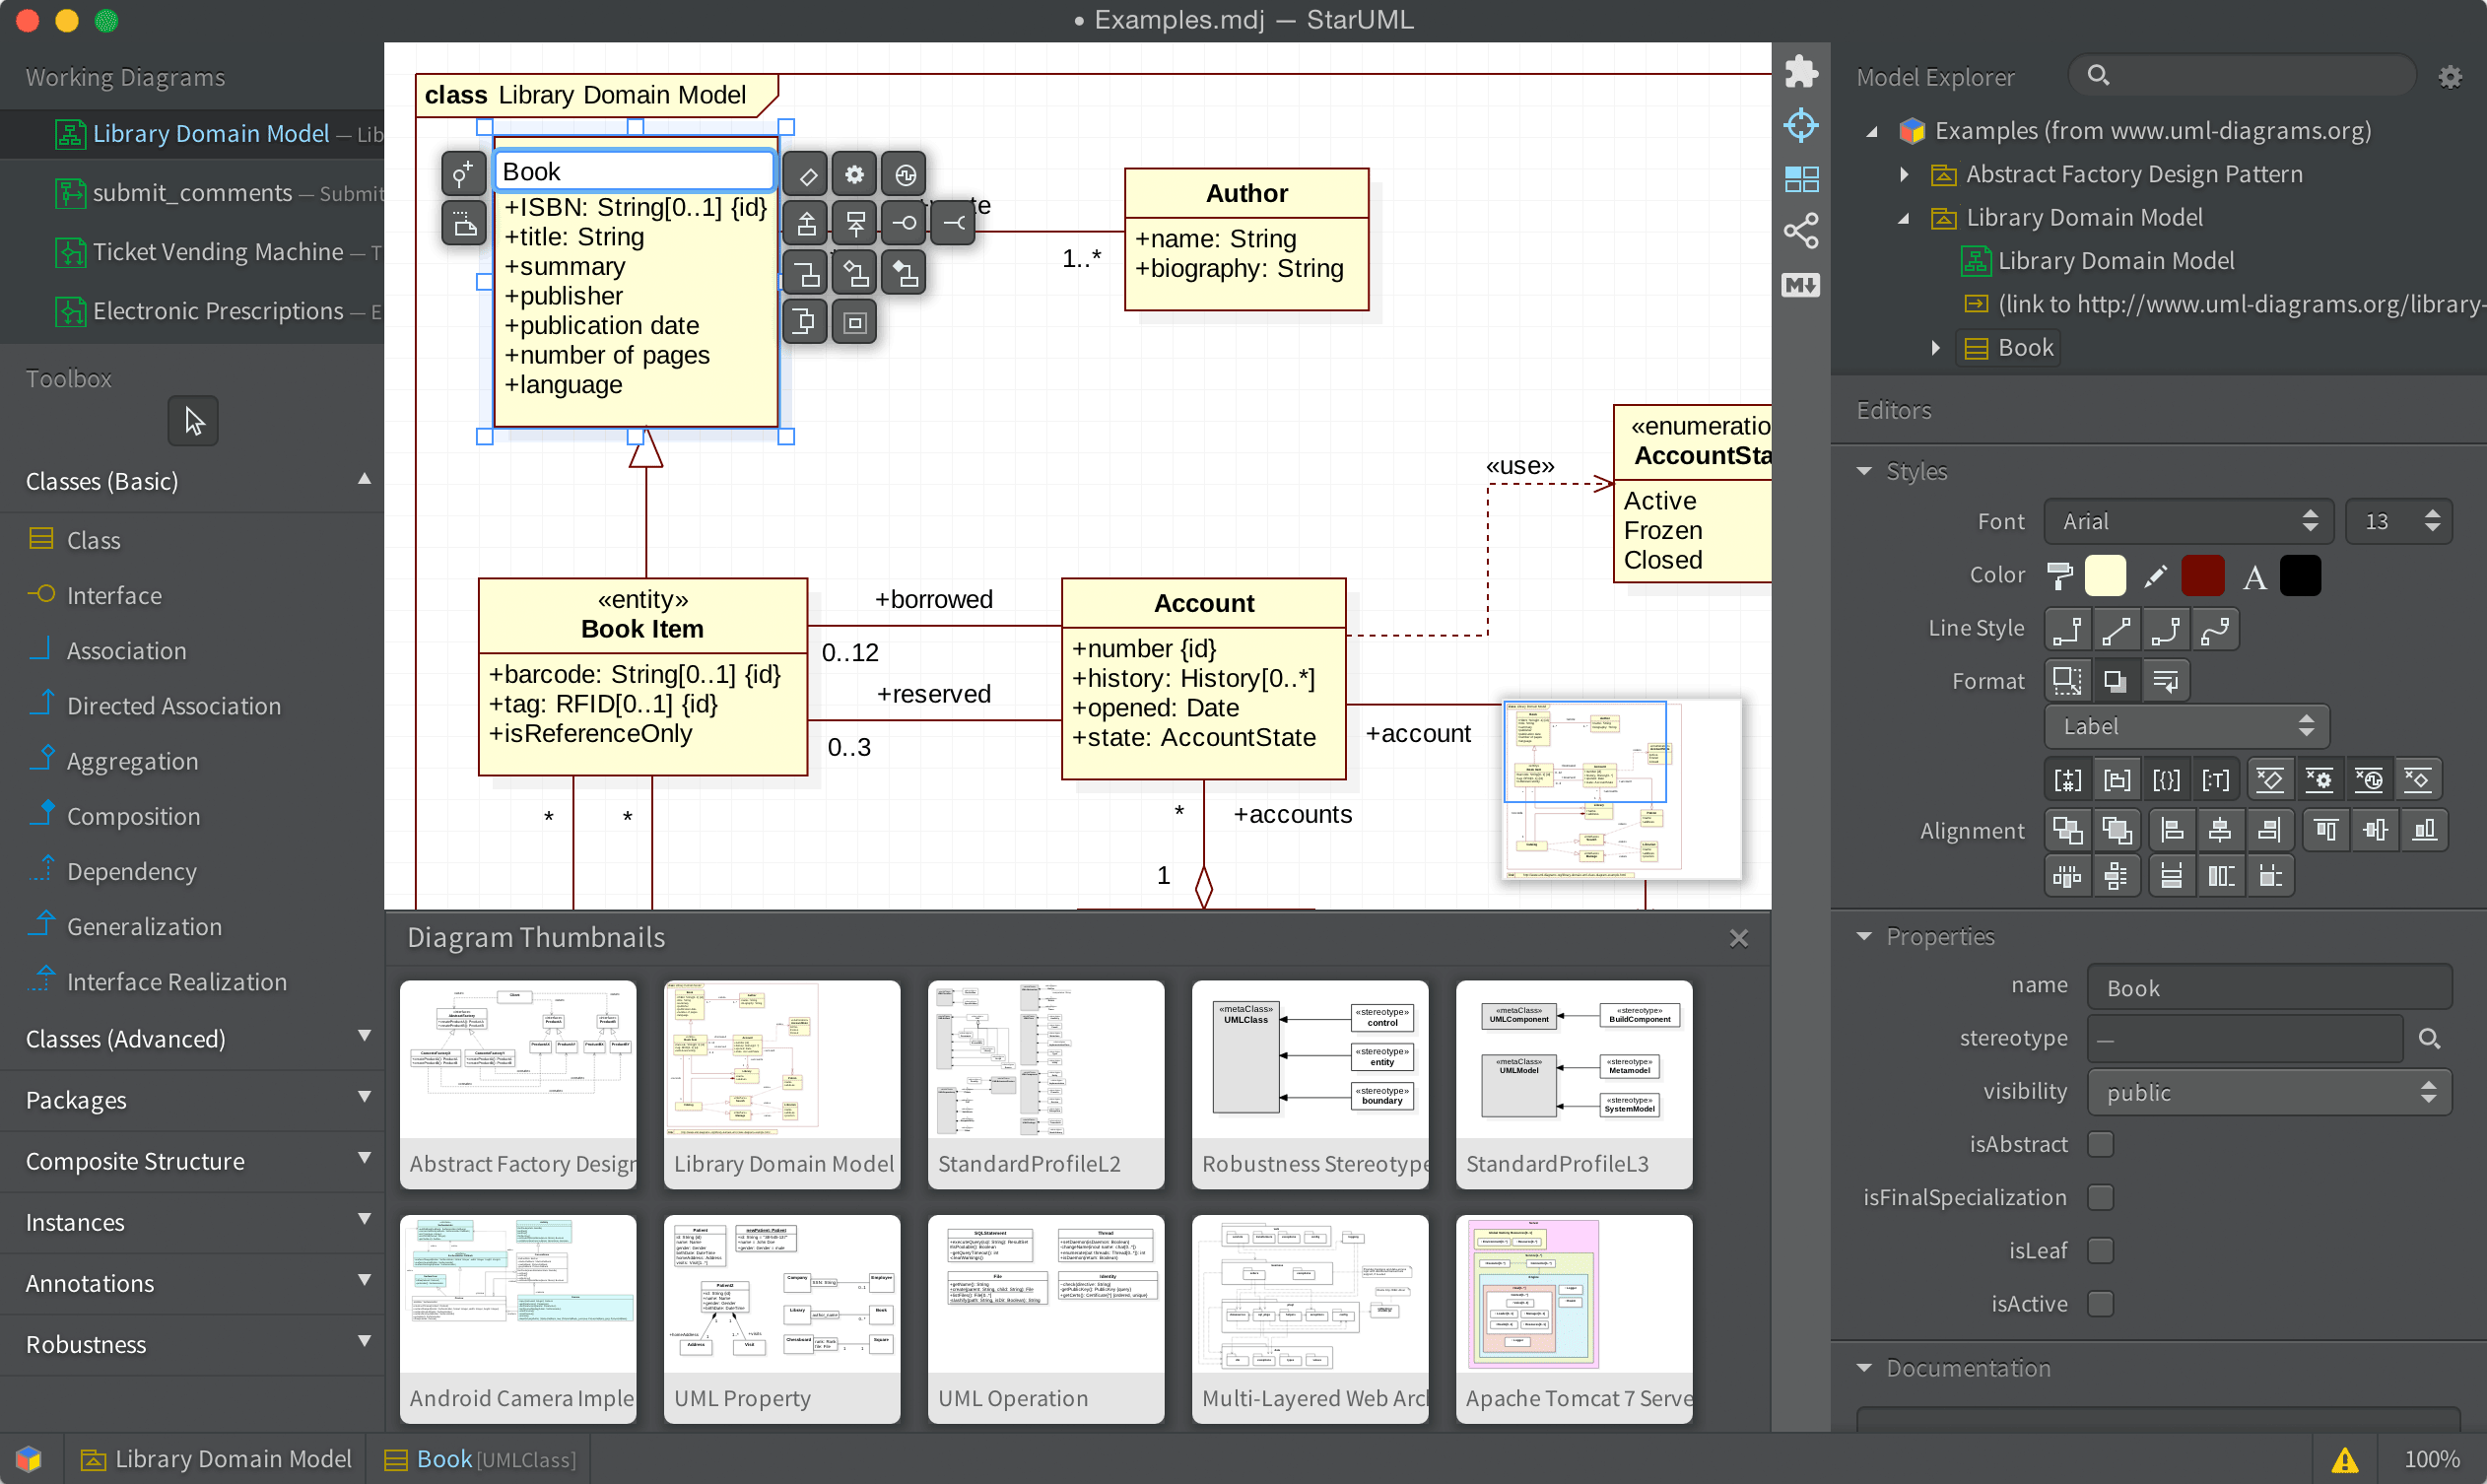
\includegraphics[width=1\textwidth]{images/starUML.png}
		\caption{Diagramma UML con StarUML} % descrizione
		\end{figure}

		
		\paragraph{SWEgo}
		\label {sec:SWEgo}
		\mbox{}\\
		SWEgo è l'applicativo web scelto dal gruppo per il tracciamento dei requisiti. Offre molti servizi, come:
		\begin{itemize}
			\item Tracciamento Use Case - requisiti:\\
			Tracciare un requisito serve a spiegare qual è l'origine di tale requisito e garantirne la necessità e la sufficienza. Il tracciamento è l'incontro tra i bisogni del proponente e dei requisiti.
			\item Generazione automatica dei diagrammi dei Casi d'Uso utilizzando PlantUML:\\
			SWEgo genera gli Use Case, dei diagrammi che esprimono un comportamento del sistema, offerto o desiderato, sulla base dei suoi risultati osservabili.
			\item Visualizzazione grafici che indicano la copertura dei requisiti: \\
			SWEgo permette di visualizzare le percentuali di copertura dei requisiti in tempo reale grazie a dei semplici grafici a torta.
		\end{itemize}
		\begin{figure}[h]
		\label{figuraSwego}
		\centering 
		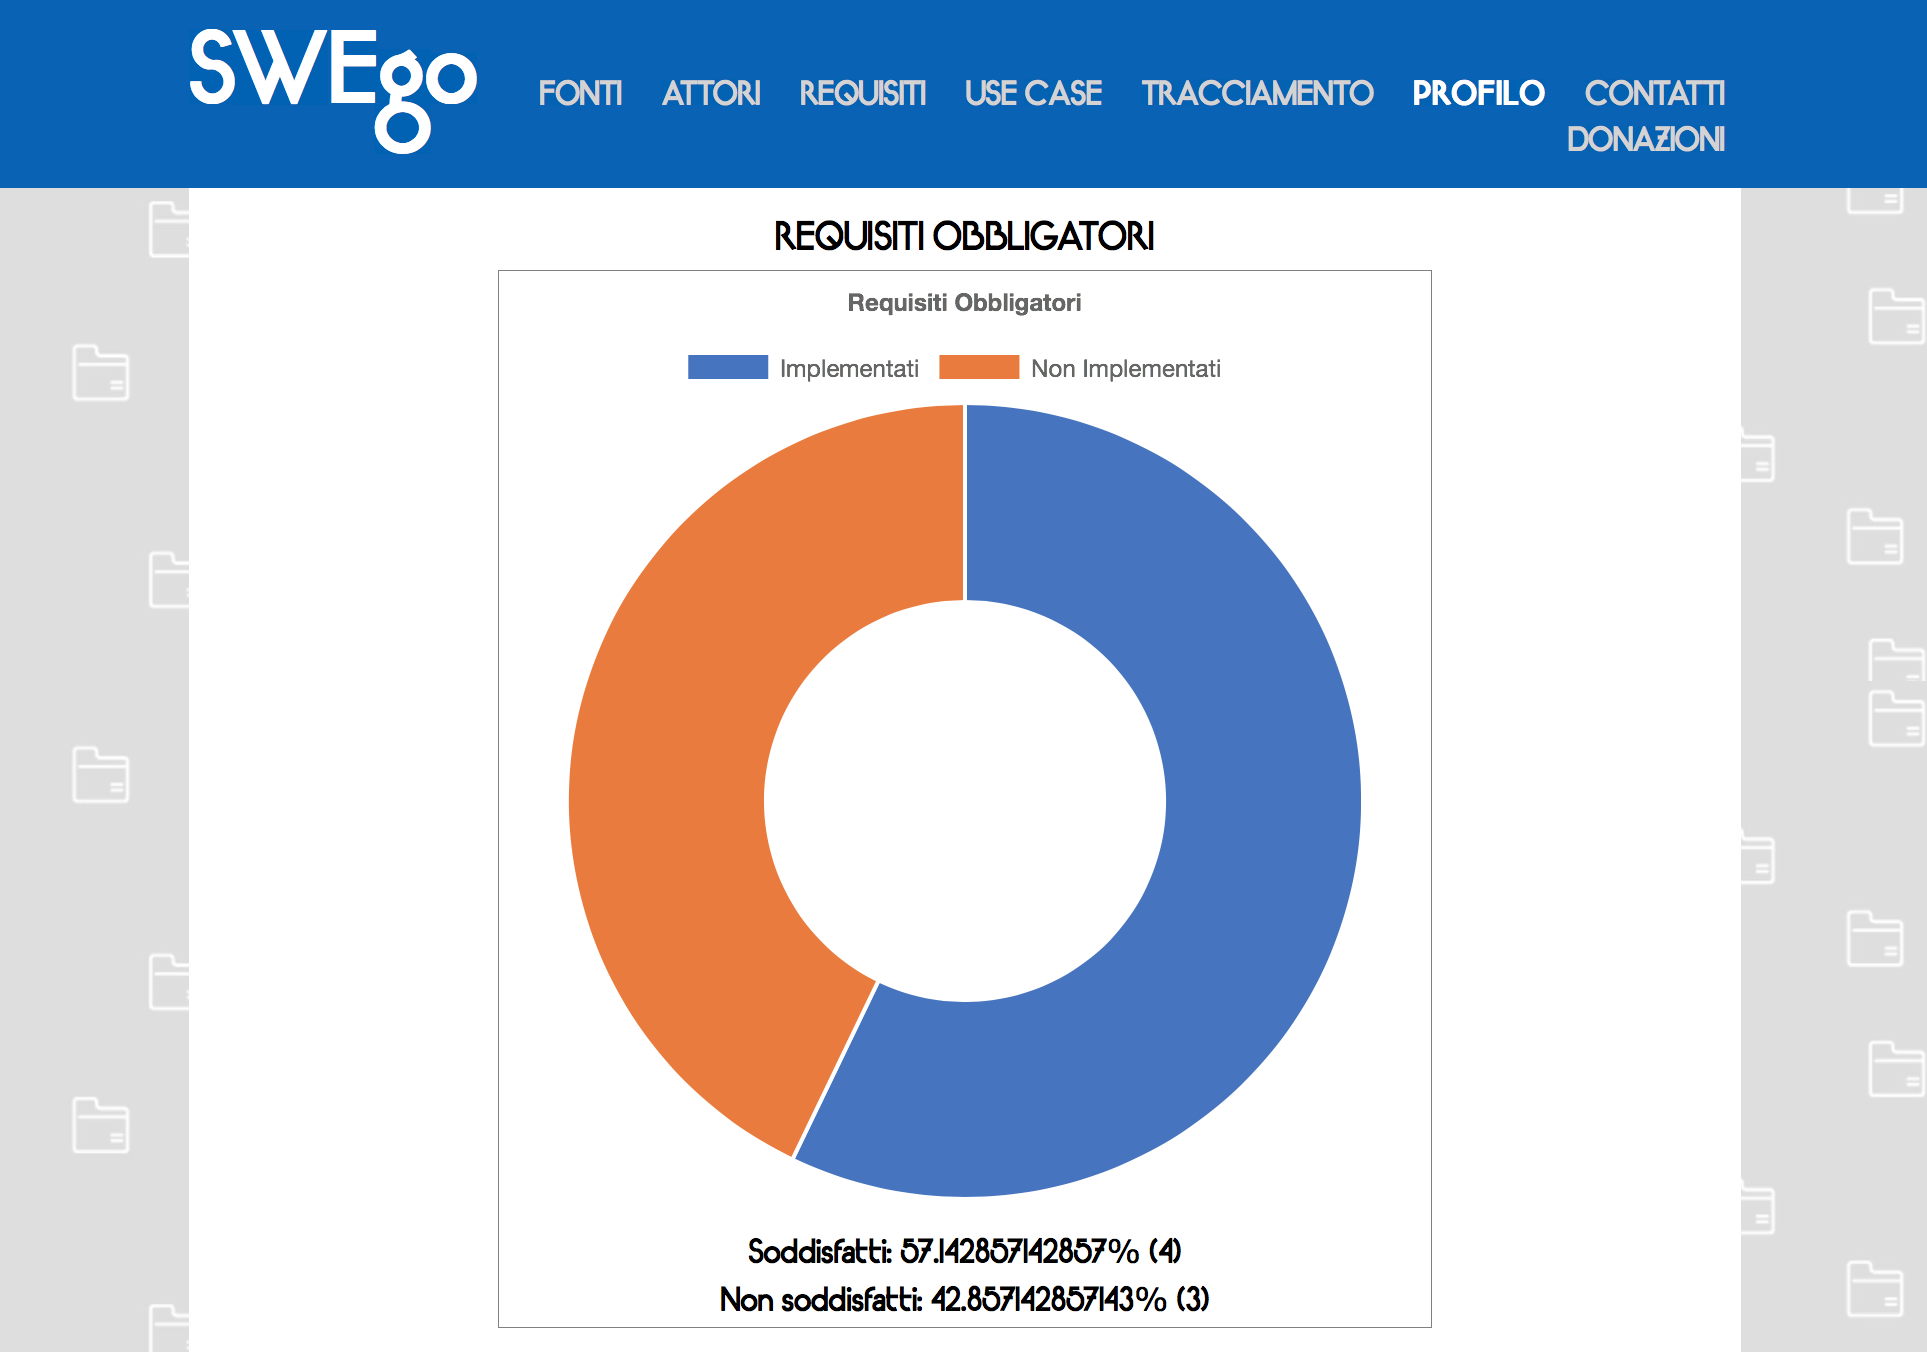
\includegraphics[width=1\textwidth]{images/swego1.png}
		\caption{Copertura requisiti con Swego} % descrizione
		\end{figure}
	
	\begin{figure}[h]
	\label{figuraSwego}
	\centering 
	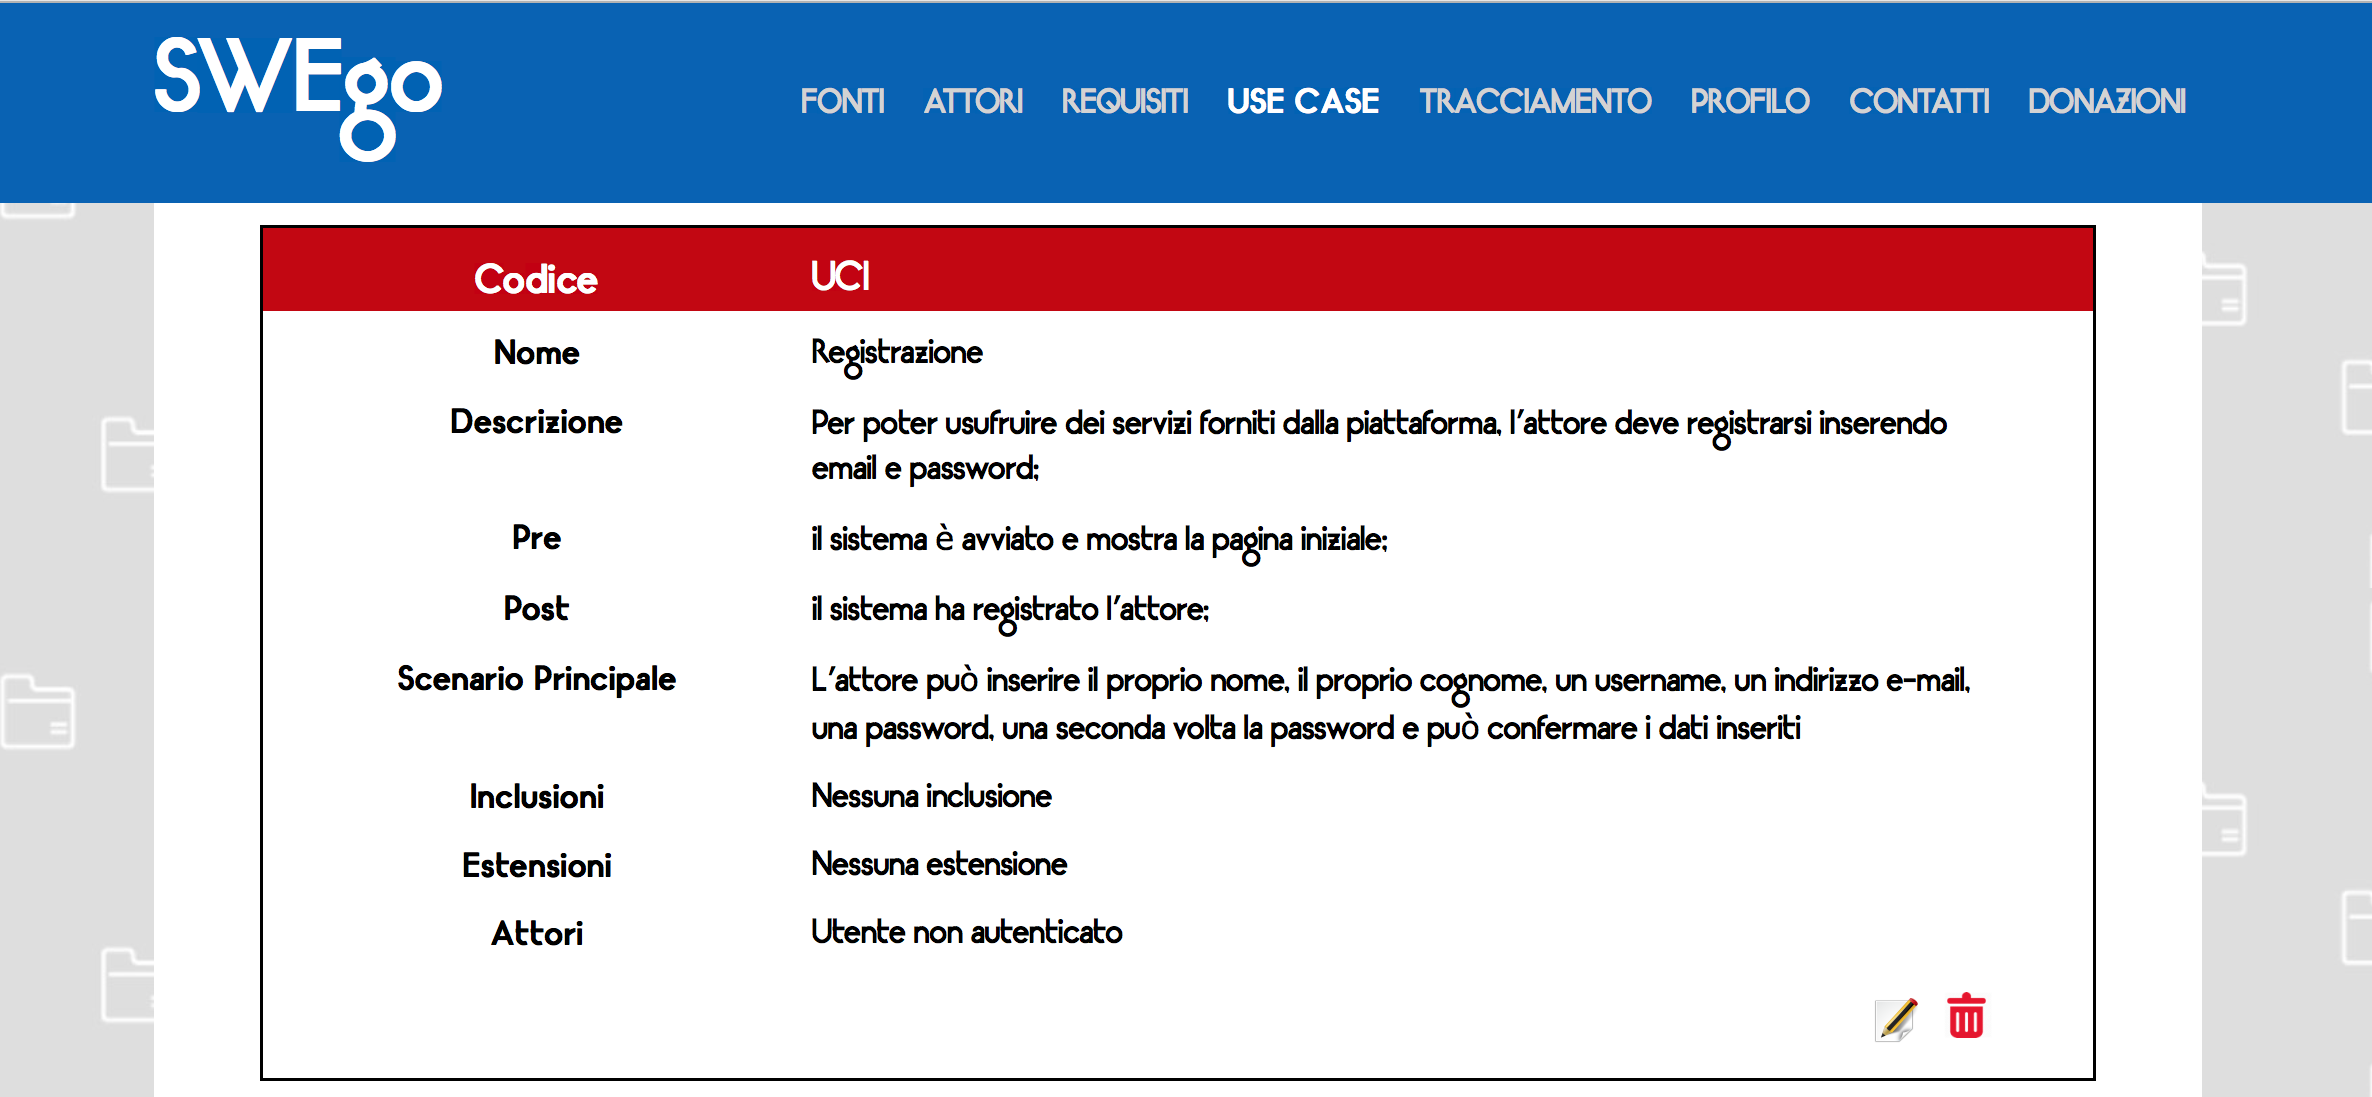
\includegraphics[width=1\textwidth]{images/swego2.png}
	\caption{Use Case con Swego} % descrizione
	\end{figure}


	
	\paragraph{Atom}
	\label{sec:Atom}
	\mbox{}\\
	Atom è un $ide_G$ di ultima generazione, sviluppato da GitHub. E' un editor potente,
	$cross platform_G$ e si integra perfettamente con tutte le tecnologie e strumenti che abbiamo deciso di utilizzare.
	Offre inoltre un vastissimo numero di $plugin_G$ grazie al grande supporto della comunità open source che lo sviluppa.
	
	\begin{figure}[h]
		\label{Atom}
		\centering 
		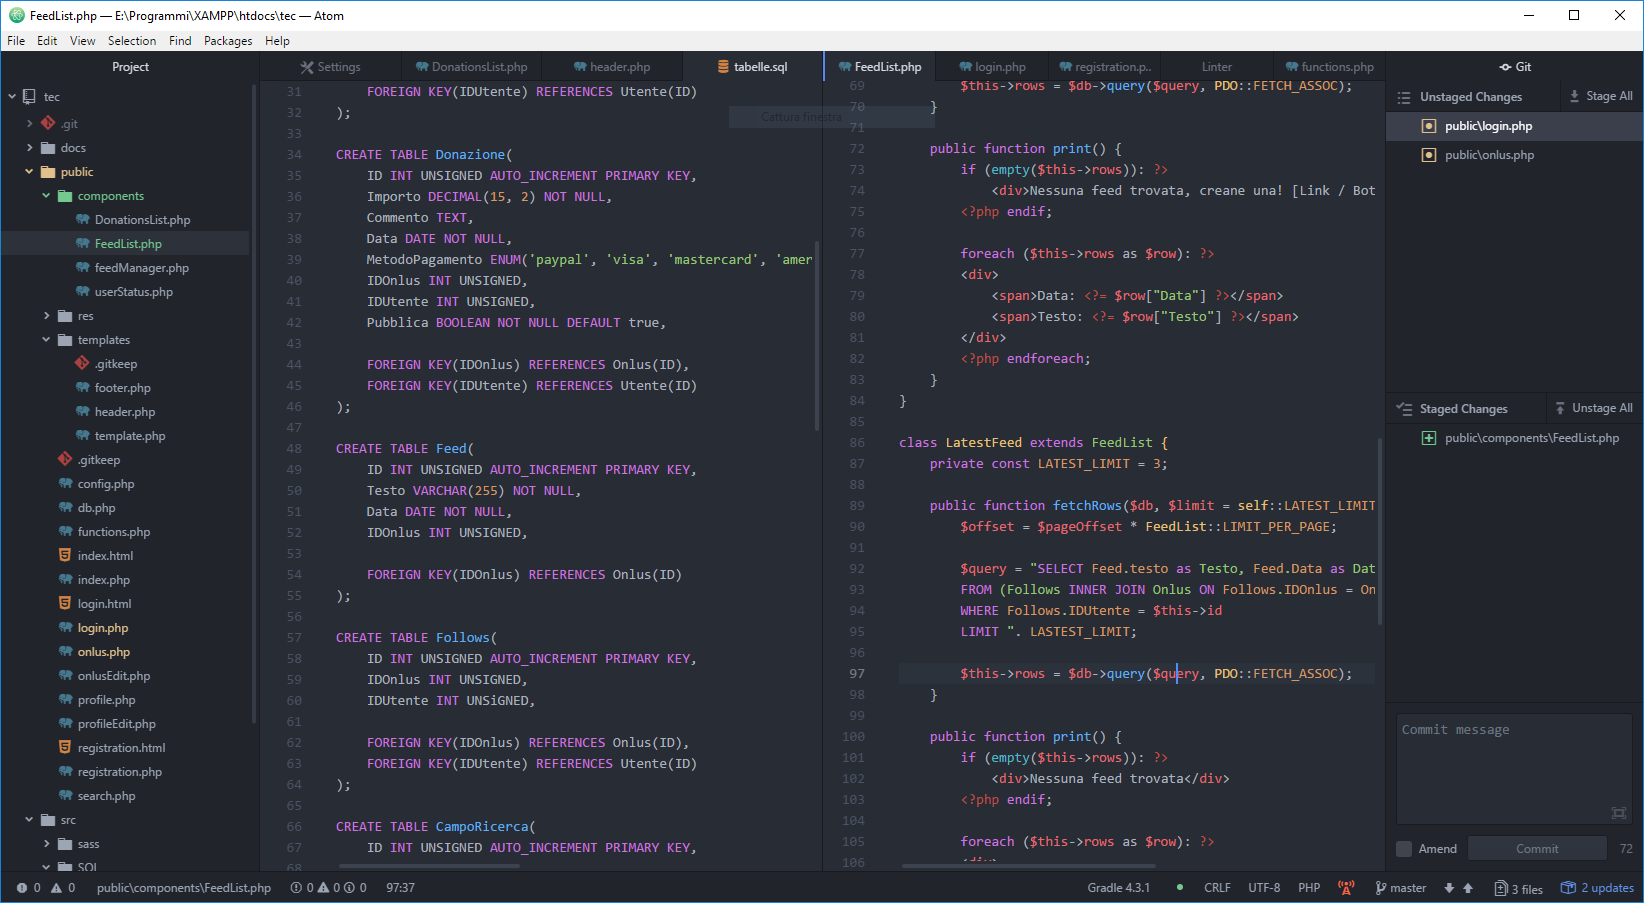
\includegraphics[width=1\textwidth]{images/atom.png}
		\caption{Interfaccia grafica di Atom} % descrizione
	\end{figure}
	
			
